\documentclass{stacsthesis}

%
% Packages
%
\usepackage[english]{babel}
\usepackage{graphicx}
\usepackage{soul}
% if the \hl command does not work for a command, register it here
\soulregister{\cite}{7}
\soulregister{\ref}{7}
\soulregister{\pageref}{7}
\soulregister{\url}{7}
\usepackage{color}
\usepackage{tabulary}
\usepackage{booktabs}
\usepackage{enumitem}
\usepackage{pifont}
\usepackage[nointegrals]{wasysym}
\usepackage{syntax}
\usepackage{textcomp}
\usepackage[font=small,labelfont=bf,skip=16pt]{caption}
\usepackage{hyperref}
\hypersetup{
    colorlinks=true,
    linkcolor=black,
    citecolor=black,
    filecolor=black,
    urlcolor=black
}

\usepackage[toc,acronym,nonumberlist,nomain]{glossaries-extra}
\setabbreviationstyle[acronym]{long-short}
\usepackage{natbib}
\usepackage{algorithm}
\usepackage{algorithmic}
\usepackage{multirow}
\usepackage{float}
\usepackage{amsfonts,amssymb}
\usepackage{silence}
\usepackage{svg}
\usepackage{tikz}
% % the command can make \mathcal better
\usepackage[cal=cm]{mathalpha}
\WarningFilter{latexfont}{Font shape}
% for those whole page pdf, use this line to make them have headers
\includepdfset{pagecommand={\thispagestyle{stacs-pg}}}
%
% Compiler warnings
%
\hfuzz=10pt
\vfuzz=10pt
\hbadness=10000
\vbadness=10000

%
% Configure caption and sub-caption styles
%
% \newsubfloat{figure}
\captionnamefont{\bfseries\small}
\captiontitlefont{\small}
\subcaptionlabelfont{\bfseries\footnotesize}
\subcaptionfont{\footnotesize}

%
% Customise titles names
%
\bibtitle{References}

%
% Customise toc
%
\maxtocdepth{subsection}

%
% Customise glossary
%
\renewcommand*{\glspostdescription}{}				% Remove dot at the end of glossary items
\makeglossaries								% Generate glossary

%
% Chapter and page style
%
\chapterstyle{stacs-chap}
\pagestyle{stacs-pg}

%
% Control word hyphenation
%
\hyphenpenalty=512
\tolerance=1024
\emergencystretch=4pt
\hyphenation{
	arti-ficial com-puter imple-ment imple-men-tation imple-men-ting frame-work
	Java
}

%
% Title page
%
\begin{document}
\hypersetup{pageanchor=false}
\title{Building Trustworthy Computer Vision: Adversarial Techniques for Robustness Assessment and Misuse Prevention}
\author{\href{mailto:zg34@st-andrews.ac.uk}{Zhongliang Guo}}
\degree{Doctor of Philosophy (PhD)}
\submittextA{This thesis is submitted in partial fulfilment for the degree of}
\submittextB{at the University of St Andrews}
\submitdate{April 2025}


% if call titlepagepdf, will ignore the above, this command is working for the titlepage pdf generated from MySaint.
\titlepagepdf{prologue/pdfs/titlepage.pdf}
\maketitle

%
% Prologue
%
% feel free to choose the declaration, I emailed the registry, both ways are fine, but personally I prefer to use the university provided word file, manually convert it to pdf.
% \begin{declaration}
\subsection*{Candidate's Declaration}
I, \hl{[Student Name]}, do hereby certify that this thesis, submitted for the degree of PhD, which is approximately \hl{[number of words]} words in length, has been written by me, and that it is the record of work carried out by me, or principally by myself in collaboration with others as acknowledged, and that it has not been submitted in any previous application for any degree. I confirm that any appendices included in my thesis contain only material permitted by the 'Assessment of Postgraduate Research Students' policy.

I was admitted as a research student at the University of St Andrews in \hl{[Month Year]}. % e.g., October 2022

I received funding from an organization or institution and have acknowledged the funder(s) in the full text of my thesis.
\vspace{24pt}

\hspace{13em}\hl{[Student Name]}\\
Date: \hl{17 April 2025} \hspace{4em} Signature of candidate
\vspace{-2.0cm}
\begin{figure}[H]
\hspace{25em}

\includegraphics[height=2cm]{prologue/signatures/student-sig.png}
\end{figure}


\subsection*{Supervisor's Declaration}
I hereby certify that the candidate has fulfilled the conditions of the Resolution and Regulations appropriate for the degree of PhD in the University of St Andrews and
that the candidate is qualified to submit this thesis in application for that degree. I confirm that any appendices included in the thesis contain only material permitted by the `Assessment of Postgraduate Research Students' policy.
\vspace{24pt}

\hspace{13em}\hl{[Supervisor Name]}\\
Date: \hl{17 April 2025} \hspace{4em} Signature of supervisor
\vspace{-2.0cm}
\begin{figure}[H]
\hspace{25em}

\includegraphics[height=2cm]{prologue/signatures/supervisor-sig.png}
\end{figure}

\newpage
\subsection*{Permission for publication}
In submitting this thesis to the University of St Andrews we understand that we are giving permission for it to be made available for use in accordance with the regulations of the University Library for the time being in force, subject to any
copyright vested in the work not being affected thereby. We also understand, unless exempt by an award of an embargo as requested below, that the title and the abstract will be published, and that a copy of the work may be made and supplied to any bona fide library or research worker, that this thesis will be electronically accessible for personal or research use and that the library has the right to migrate this thesis into new electronic forms as required to ensure continued access to the thesis.

I, Zhongliang Guo, confirm that my thesis does not contain any third-party material that requires copyright clearance.

The following is an agreed request by candidate and supervisor regarding the publication of this thesis:

% \vspace{8pt}
% \subsubsection*{Printed copy}
% No embargo on print copy.
\vspace{8pt}

\subsubsection*{Electronic copy}
No embargo on electronic copy.
\vspace{48pt}

\hspace{13em}\hl{[Student Name]}\\
Date: \hl{17 April 2025} \hspace{4em} Signature of candidate
\vspace{-2.0cm}
\begin{figure}[H]
\hspace{25em}

\includegraphics[height=2cm]{prologue/signatures/student-sig.png}
\end{figure}

\hspace{13em}\hl{[Supervisor Name]}\\
Date: \hl{17 April 2025} \hspace{4em} Signature of supervisor
\vspace{-2.0cm}
\begin{figure}[H]
\hspace{25em}

\includegraphics[height=2cm]{prologue/signatures/supervisor-sig.png}
\end{figure}

\newpage
\subsubsection*{Underpinning Research Data or Digital Outputs}
\subsubsection*{Candidate's declaration}
I, \hl{[Student Name]}, hereby certify that no requirements to deposit original research data or digital outputs apply to this thesis and that, where appropriate, secondary data used have been referenced in the full text of my thesis.

\vspace{48pt}

\hspace{13em}\hl{[Student Name]}\\
Date: \hl{17 April 2025} \hspace{4em} Signature of candidate
\vspace{-2.0cm}
\begin{figure}[H]
\hspace{25em}

\includegraphics[height=2cm]{prologue/signatures/student-sig.png}
\end{figure}

\end{declaration}  % this allows you to sign the document by png inside of the latex
% if your declaration is over 3 pages, just edit pages={1,2,3} to pages={1,2,3,4,5} or more
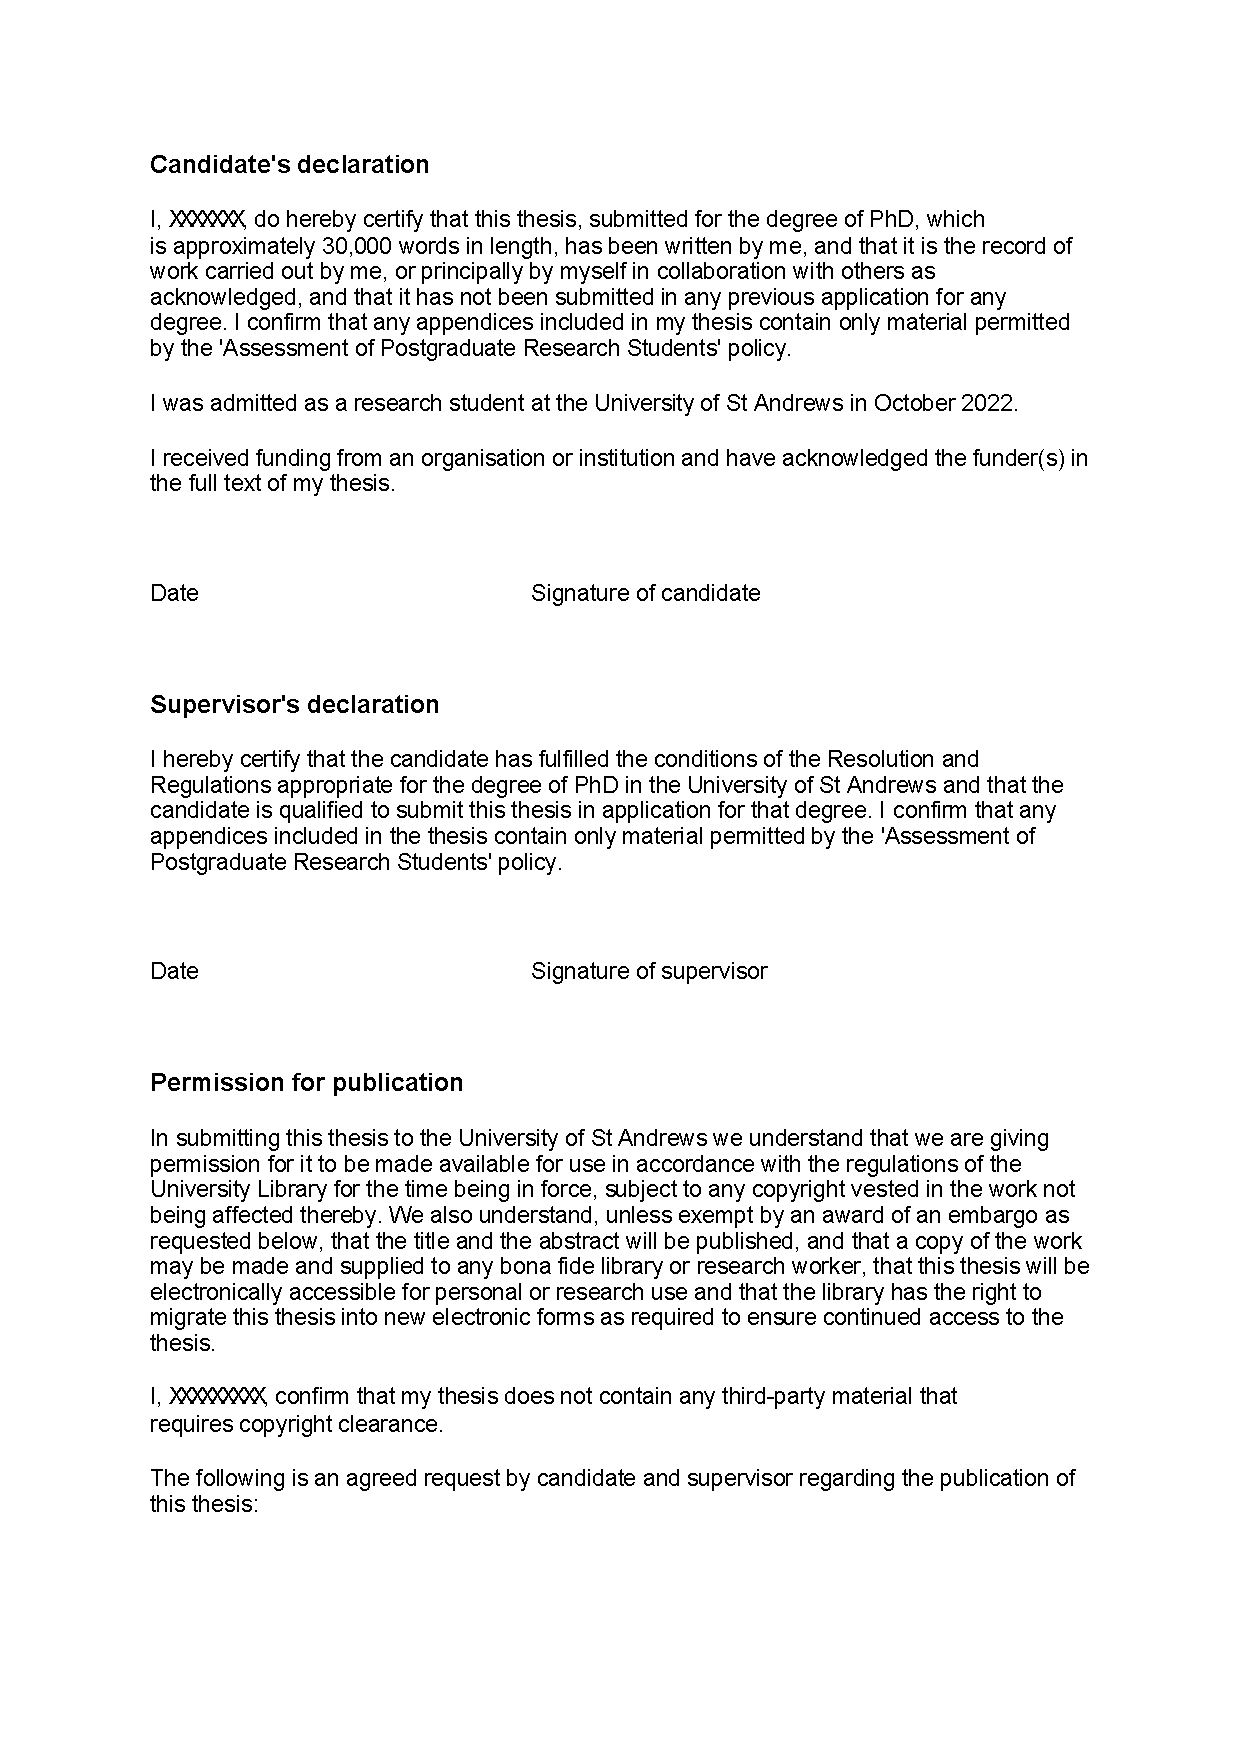
\includepdf[pages={1,2,3}, pagecommand={\thispagestyle{empty}}, scale=1]{prologue/pdfs/declarations.pdf}  % this require your supervisor and you to sign the pdf.

\begin{abstract}
    Abstract goes here.
    
\end{abstract}
\begin{acknowledgement}
Acknowledgement goes here.

\vspace{2em}
\section*{Funding} % delete it if you do not have funding
This work was supported by the \hl{XXX [Grant Number]}.
\end{acknowledgement}
\newacronym{ai}{AI}{Artificial Intelligence}
\newacronym{dl}{DL}{Deep Learning}
\newacronym{ml}{ML}{Machine Learning}
\newacronym{nn}{NN}{Neural Network}
\newacronym{cnn}{CNN}{Convolutional Neural Network}


%
% Tables of contents/figures/tables and glossary
%
\cleardoublepage
\hypersetup{pageanchor=true}
\pagenumbering{roman}
\tableofcontents
\newpage\listoffigures
\newpage\listoftables
\printglossaries

%
% Mainmatter properties
%
\mainmatter
\onehalfspacing
\pagenumbering{arabic}
\setlength{\parskip}{3mm}
\setlength{\parindent}{0mm}
\setlist[enumerate]{leftmargin=*,labelsep=0.8em,topsep=0em,parsep=0.6em}
\setlist[itemize]{leftmargin=*,labelsep=1.0em,topsep=0em,parsep=0.6em,label=\normalsize\textbullet}
\newenvironment{itemize*}			% Itemising environment for single-lined items
	{\begin{itemize}					% Interline spacing has been adjusted in this case to
    		\setlength{\itemsep}{0.016em}}	% make the itemised text look more consistent with the rest
     	{\end{itemize}}

%
% Graphics directories
%
\graphicspath{
	{chap1/}
	{chap-example/}
	{appA/}
	{appB/}
        {appC/}
}

%
% Chapters
%
\chapter{Introduction}
This is a PhD/Master thesis template for the University of St Andrews, modified from the Lakshithade Silva's GitHub repository\footnote{\url{https://github.com/LakshithadeSilva/stacs-thesis}}. I solved some warnings in the original repo, and added some features and more \LaTeX usage examples. I will give the necessary explanation in the following sections.

\section{Added Features \& Solved Warnings}
\subsection{Flexible Title Page}
When you declare the intention of submitting the thesis, the MySaint will automatically generate a title page pdf. Some people may want to use this pdf rather than the template in this \LaTeX project.

The usage is simple:
\begin{itemize}
    \item If you want to use the pdf provided by MySaint:\\
    replace the \boxed{prologue/pdfs/titlepage.pdf} to your own title page
    \item If you want to use the tile page of \LaTeX:
    Delete or comment the \textbf{line 111}\\
    \verb|\| titlepagepdf\{prologue/pdfs/titlepage.pdf\} of \boxed{thesis.tex}
\end{itemize}

\subsection{Flexible Declaration}
Same as the title page, MySaint also provides the declaration template. Please refer to the comments in \textbf{line 117-119} of \boxed{thesis.tex}.

\subsection{Ethics Approval}
These years the School of Computer Science tends to more stringent ethical assessment, even you only use the open-source dataset, you need to apply the ethical approval and attach it in the thesis. I added an example in the Appendix~\ref{app:c}.

\subsection{In-Math Font}
The in-math font of the original \LaTeX\ template looks a little bit weird for me, which does not align with the convention of AI conference, so I changed it somehow.

\subsection{Box and Color of the Hyperlink}
Same as the in-math font, I changed it.

\subsection{Acronyms Warnings}
The original \LaTeX\ template has some warnings about glossary/acronyms, it is fine to compile but annoying for me, so I correct them somehow.

\section{More Examples of \LaTeX\  Usage}
\subsection{Acronyms}
You should define acronyms in the \boxed{prologue/glossarys.tex} first, then use it. Here are some usages:
\begin{itemize}
    \item When you first time call \verb|\|gls\{ai\}, it will appear: \gls{ai}, i.e., \hl{full and abbreviated}.
    \item Same as the \verb|\|glspl\{ml\}: \glspl{ml}, ``pl'' refers to the plurality.
    \item afterwards, when you call \verb|\|gls\{ai\}, it appears \gls{ai}. To make it \hl{full and abbreviated}, use \glsxtrfull{ai} or \glsxtrfullpl{ai}.
\end{itemize}

\subsection{Support of the Formula in Section Title}
If I remember it correctly, this template does not support to have the math symbol in the section title, I solved it somehow. Please refer to Chapter~\ref{math:in:title}.

\subsection{Solution for the Long Chapter Tile or Float Caption}
Some chapter title is quite long and it's ugly in the table of content, please see the \boxed{chap-example/doc.tex} (Chapter~\ref{chap:ex}).
\chapter[Title in the table of content]{This is a very Long Title This is a very Long Title This is a very Long Title This is a very Long Title}\label{chap:ex}

\section{Long Caption}
Same as the float:
\begin{table}[ht]
\centering
\caption[Ablation study on learning rate]{Ablation study on $\alpha$. Ablation study on $\alpha$. Ablation study on $\alpha$. Ablation study on $\alpha$. Ablation study on $\alpha$. Ablation study on $\alpha$. Ablation study on $\alpha$. Ablation study on $\alpha$. }
\resizebox{\textwidth}{!}{
\begin{tabular}{cccccccccccc}
\hline
\multirow{2}{*}{prompt}                  & \multirow{2}{*}{$\alpha$} & \multicolumn{2}{c}{PSNR$\uparrow$}                                        & \multicolumn{2}{c}{FID$\downarrow$}                                         & \multicolumn{2}{c}{SSIM$\uparrow$}                                          & \multicolumn{2}{c}{LPIPS$\downarrow$}                                       & \multicolumn{2}{c}{ACDM$\downarrow$}                   \\
                                         &                           & SD14                                & SD15                                & SD14                                 & SD15                                 & SD14                                 & SD15                                 & SD14                                 & SD15                                 & SD14                                 & SD15            \\ \hline
\multicolumn{1}{c|}{\multirow{3}{*}{P1}} & \multicolumn{1}{c|}{1}    & \multicolumn{1}{c|}{18.18}          & \multicolumn{1}{c|}{18.18}          & \multicolumn{1}{c|}{137.44}          & \multicolumn{1}{c|}{134.12}          & \multicolumn{1}{c|}{0.4563}          & \multicolumn{1}{c|}{0.4576}          & \multicolumn{1}{c|}{0.6137}          & \multicolumn{1}{c|}{0.6119}          & \multicolumn{1}{c|}{0.1075}          & 0.1080          \\
\multicolumn{1}{c|}{}                    & \multicolumn{1}{c|}{2}    & \multicolumn{1}{c|}{\textbf{18.02}} & \multicolumn{1}{c|}{\textbf{18.02}} & \multicolumn{1}{c|}{\textbf{139.11}} & \multicolumn{1}{c|}{\textbf{135.32}} & \multicolumn{1}{c|}{0.4441}          & \multicolumn{1}{c|}{0.4453}          & \multicolumn{1}{c|}{\textbf{0.6188}} & \multicolumn{1}{c|}{\textbf{0.6171}} & \multicolumn{1}{c|}{\textbf{0.1106}} & \textbf{0.1110} \\
\multicolumn{1}{c|}{}                    & \multicolumn{1}{c|}{4}    & \multicolumn{1}{c|}{18.43}          & \multicolumn{1}{c|}{18.44}          & \multicolumn{1}{c|}{132.79}          & \multicolumn{1}{c|}{132.77}          & \multicolumn{1}{c|}{\textbf{0.4408}} & \multicolumn{1}{c|}{\textbf{0.4419}} & \multicolumn{1}{c|}{0.6057}          & \multicolumn{1}{c|}{0.6049}          & \multicolumn{1}{c|}{0.0961}          & 0.0966          \\ \hline
\multicolumn{1}{c|}{\multirow{3}{*}{P2}} & \multicolumn{1}{c|}{1}    & \multicolumn{1}{c|}{16.85}          & \multicolumn{1}{c|}{16.82}          & \multicolumn{1}{c|}{70.40}           & \multicolumn{1}{c|}{68.52}           & \multicolumn{1}{c|}{0.4448}          & \multicolumn{1}{c|}{0.4445}          & \multicolumn{1}{c|}{0.5956}          & \multicolumn{1}{c|}{0.5938}          & \multicolumn{1}{c|}{0.1131}          & 0.1142          \\
\multicolumn{1}{c|}{}                    & \multicolumn{1}{c|}{2}    & \multicolumn{1}{c|}{\textbf{16.74}} & \multicolumn{1}{c|}{\textbf{16.70}} & \multicolumn{1}{c|}{\textbf{70.59}}  & \multicolumn{1}{c|}{\textbf{69.04}}  & \multicolumn{1}{c|}{0.4336}          & \multicolumn{1}{c|}{0.4329}          & \multicolumn{1}{c|}{\textbf{0.6005}} & \multicolumn{1}{c|}{\textbf{0.5990}} & \multicolumn{1}{c|}{\textbf{0.1156}} & \textbf{0.1167} \\
\multicolumn{1}{c|}{}                    & \multicolumn{1}{c|}{4}    & \multicolumn{1}{c|}{17.10}          & \multicolumn{1}{c|}{17.08}          & \multicolumn{1}{c|}{66.88}           & \multicolumn{1}{c|}{65.54}           & \multicolumn{1}{c|}{\textbf{0.4330}} & \multicolumn{1}{c|}{\textbf{0.4327}} & \multicolumn{1}{c|}{0.5887}          & \multicolumn{1}{c|}{0.5863}          & \multicolumn{1}{c|}{0.1018}          & 0.1026          \\ \hline
\multicolumn{1}{c|}{\multirow{3}{*}{P3}} & \multicolumn{1}{c|}{1}    & \multicolumn{1}{c|}{16.86}          & \multicolumn{1}{c|}{16.91}          & \multicolumn{1}{c|}{155.70}          & \multicolumn{1}{c|}{152.69}          & \multicolumn{1}{c|}{0.4330}          & \multicolumn{1}{c|}{0.4323}          & \multicolumn{1}{c|}{0.6165}          & \multicolumn{1}{c|}{0.6171}          & \multicolumn{1}{c|}{0.1052}          & 0.1053          \\
\multicolumn{1}{c|}{}                    & \multicolumn{1}{c|}{2}    & \multicolumn{1}{c|}{\textbf{16.71}} & \multicolumn{1}{c|}{\textbf{16.78}} & \multicolumn{1}{c|}{\textbf{156.47}} & \multicolumn{1}{c|}{\textbf{153.85}} & \multicolumn{1}{c|}{0.4234}          & \multicolumn{1}{c|}{0.4228}          & \multicolumn{1}{c|}{\textbf{0.6202}} & \multicolumn{1}{c|}{\textbf{0.6204}} & \multicolumn{1}{c|}{\textbf{0.1084}} & \textbf{0.1079} \\
\multicolumn{1}{c|}{}                    & \multicolumn{1}{c|}{4}    & \multicolumn{1}{c|}{17.00}          & \multicolumn{1}{c|}{17.04}          & \multicolumn{1}{c|}{140.65}          & \multicolumn{1}{c|}{139.28}          & \multicolumn{1}{c|}{\textbf{0.4198}} & \multicolumn{1}{c|}{\textbf{0.4189}} & \multicolumn{1}{c|}{0.6110}          & \multicolumn{1}{c|}{0.6108}          & \multicolumn{1}{c|}{0.0958}          & 0.0956          \\ \hline
\multicolumn{1}{c|}{\multirow{3}{*}{P4}} & \multicolumn{1}{c|}{1}    & \multicolumn{1}{c|}{17.75}          & \multicolumn{1}{c|}{17.62}          & \multicolumn{1}{c|}{\textbf{118.34}} & \multicolumn{1}{c|}{113.48}          & \multicolumn{1}{c|}{0.4138}          & \multicolumn{1}{c|}{0.4067}          & \multicolumn{1}{c|}{0.6305}          & \multicolumn{1}{c|}{0.6337}          & \multicolumn{1}{c|}{0.1021}          & 0.1036          \\
\multicolumn{1}{c|}{}                    & \multicolumn{1}{c|}{2}    & \multicolumn{1}{c|}{\textbf{17.61}} & \multicolumn{1}{c|}{\textbf{17.50}} & \multicolumn{1}{c|}{116.48}          & \multicolumn{1}{c|}{\textbf{115.41}} & \multicolumn{1}{c|}{0.4004}          & \multicolumn{1}{c|}{0.3942}          & \multicolumn{1}{c|}{\textbf{0.6361}} & \multicolumn{1}{c|}{\textbf{0.6394}} & \multicolumn{1}{c|}{\textbf{0.1051}} & \textbf{0.1067} \\
\multicolumn{1}{c|}{}                    & \multicolumn{1}{c|}{4}    & \multicolumn{1}{c|}{17.96}          & \multicolumn{1}{c|}{17.85}          & \multicolumn{1}{c|}{110.58}          & \multicolumn{1}{c|}{109.59}          & \multicolumn{1}{c|}{\textbf{0.3929}} & \multicolumn{1}{c|}{\textbf{0.3876}} & \multicolumn{1}{c|}{0.6302}          & \multicolumn{1}{c|}{0.6347}          & \multicolumn{1}{c|}{0.0918}          & 0.0927          \\ \hline
\multicolumn{1}{c|}{\multirow{3}{*}{P5}} & \multicolumn{1}{c|}{1}    & \multicolumn{1}{c|}{16.91}          & \multicolumn{1}{c|}{17.06}          & \multicolumn{1}{c|}{132.37}          & \multicolumn{1}{c|}{128.71}          & \multicolumn{1}{c|}{0.4670}          & \multicolumn{1}{c|}{0.4628}          & \multicolumn{1}{c|}{0.5989}          & \multicolumn{1}{c|}{0.6004}          & \multicolumn{1}{c|}{0.1207}          & 0.1182          \\
\multicolumn{1}{c|}{}                    & \multicolumn{1}{c|}{2}    & \multicolumn{1}{c|}{\textbf{16.81}} & \multicolumn{1}{c|}{\textbf{16.95}} & \multicolumn{1}{c|}{\textbf{134.71}} & \multicolumn{1}{c|}{\textbf{129.93}} & \multicolumn{1}{c|}{0.4568}          & \multicolumn{1}{c|}{0.4524}          & \multicolumn{1}{c|}{\textbf{0.6032}} & \multicolumn{1}{c|}{\textbf{0.6047}} & \multicolumn{1}{c|}{\textbf{0.1227}} & \textbf{0.1209} \\
\multicolumn{1}{c|}{}                    & \multicolumn{1}{c|}{4}    & \multicolumn{1}{c|}{17.18}          & \multicolumn{1}{c|}{17.33}          & \multicolumn{1}{c|}{126.82}          & \multicolumn{1}{c|}{124.19}          & \multicolumn{1}{c|}{\textbf{0.4547}} & \multicolumn{1}{c|}{\textbf{0.4516}} & \multicolumn{1}{c|}{0.5932}          & \multicolumn{1}{c|}{0.5939}          & \multicolumn{1}{c|}{0.1088}          & 0.1073          \\ \hline
\end{tabular}
}
\label{tab:ablation:alpha}
\end{table}

\newpage
\section{Math Formula \texorpdfstring{$\frac{1}{2} \alpha$}{1/2 alpha} Support in the Section Title}\label{math:in:title}
\verb|\|texorpdfstring\{formula\}\{corresponding pure text\}

\section{Citation}
Only support something like Some researchers~\cite{ho2020ddpm} $\cdots$, do not support \verb|\|citeauthor or \verb|\|citeyear.

\section{Draw Figures}
You may need to have some figures in one pdf (for faster compile), here I provide a example how I make it in \boxed{chap-example/figs/draw-figure.tex}. Please note that, you may be unable to compile if you compile the thesis before, just clean the cache or recompile from scratch. Then download it and insert it in the thesis:

\begin{figure}[htbp]
    \centering
    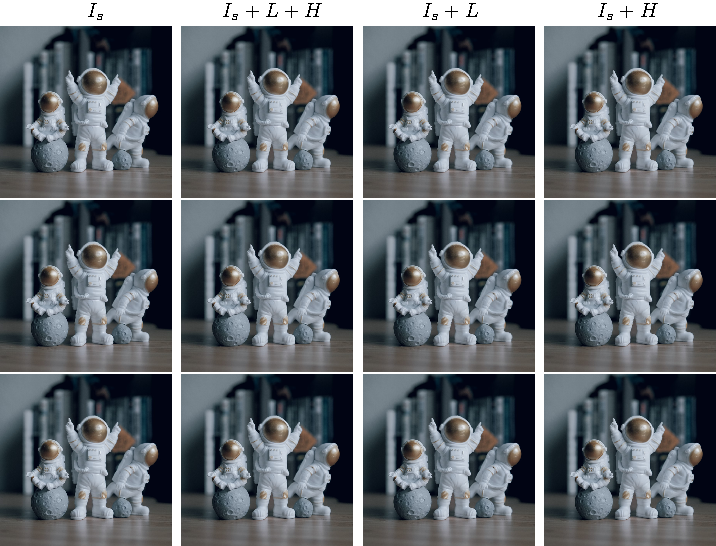
\includegraphics[width=0.6\linewidth]{chap-example/figs/example-fig.pdf}
    \caption[a figure]{long caption. long caption. long caption. long caption. long caption. long caption. long caption. long caption.}
    \label{fig:eg}
\end{figure}

\subsection{Position of the figure}
In line 17, you may notice the htbp. h=here, t=top, b=bottom, p=anywhere of the page. In some case ``h'' doesn't work, try only ``H''.

\section{Useful Tools}
\begin{itemize}
    \item Table: \url{https://tablesgenerator.com/latex_tables}
    \item Formula:
    \url{https://www.latexlive.com/}
    \item Crop pdf's blank border (Usually works for ppt made pdf): \url{https://croppdf.com/}
\end{itemize}

%
% Appendices
%
\appendix
\chapter{Miscellaneous}

\chapter{List of Publications}

\section*{Peer Reviewed Conference Contributions}
\begin{enumerate}
    \item \textbf{Chenlin Meng}, Yutong He, Yang Song, Jiaming Song, Jiajun Wu, Jun-Yan Zhu, and Stefano Ermon. SDEdit: Guided image synthesis and editing with stochastic differential equations. In \textit{International Conference on Learning Representations}, 2022.
\end{enumerate}
\nocite{meng2021sdedit}

% \clearpage

\section*{Peer Reviewed Journal Contributions}
\begin{enumerate}
    \item \textbf{Haochen Dou}, Zhenwu Dan, Peng Xu, Wei Wang, Shuning Xu, Tianyang Chen, and Hai Jin. Dynamic searchable symmetric encryption with strong security and robustness. \textit{IEEE Transactions on Information Forensics and Security}, 19:2370–2384, 2024.
\end{enumerate}
\nocite{dou2024dynamic}

% \clearpage

\section*{Preprints Under Review}
\begin{enumerate}
    \item \textbf{Christina M Funke}, Leon A Gatys, Alexander S Ecker, and Matthias Bethge. Synthesising dynamic textures using convolutional neural networks. \textit{arXiv preprint arXiv:1702.07006}, 2017.
\end{enumerate}
\nocite{funke2017synthesising}
\chapter{The Ethics Approval}\label{app:c}
This Appendix is to show any ethical concerns about this project.

According to the regulations of UTREC\footnote{\url{https://www.st-andrews.ac.uk/utrec/}} (University Teaching and Research Ethics Committee), there is no ethical issues raised by this thesis.

The ethical approval document will be attached in the following pages.

\newpage
% replace it with your ethic approval if it's available

\includepdf[pages={1}, pagecommand={\thispagestyle{empty}}, scale=1]{appC/ethics.pdf}
%
% Bibliography
%
\bibliographystyle{plain}
\bibliography{thesis}

\end{document}
